% section 2 Proposal
In this chapter, the fundamental macroscopic concepts of superconductivity, Meissner effect, ferrormagnetism,
and the modern high temperature superconductor tape are described in detail.
With only limited acknowledge of Maxwell equation is assumed, readers who are new to this region should be able to understand unproblematically.
For advanced readers who is familiar to superconductivity, you are welcome to skip to the magnetic cloak parts.

In the later sections of this chapter, we first give an introduction on the conventional magnetic cloak,
how the concept works and the potential issue occured.
Then the description of the proposed new Electromagnetic Induction type magnetic cloak follows.


\newpage
\subsection{Superconductor}
Since its first discover in 1911, superconductor materials have been surprising scientists with the rapid improvement year after year.
In 1911, short after the liquefaction of helium had been achieved, Kamerlingh Onnes found that the electrical resistance of mercury dropped extremely under a low temperature of 4.2 K \cite{2_1}.
This phenomanen is later discovered to appear in several metals, and is named "superconductivity" by Kamerlingh.
The result of the experiment conducted on mercury is shown in Fig. \ref{fig:mercury}.
\begin{figure}[H]
  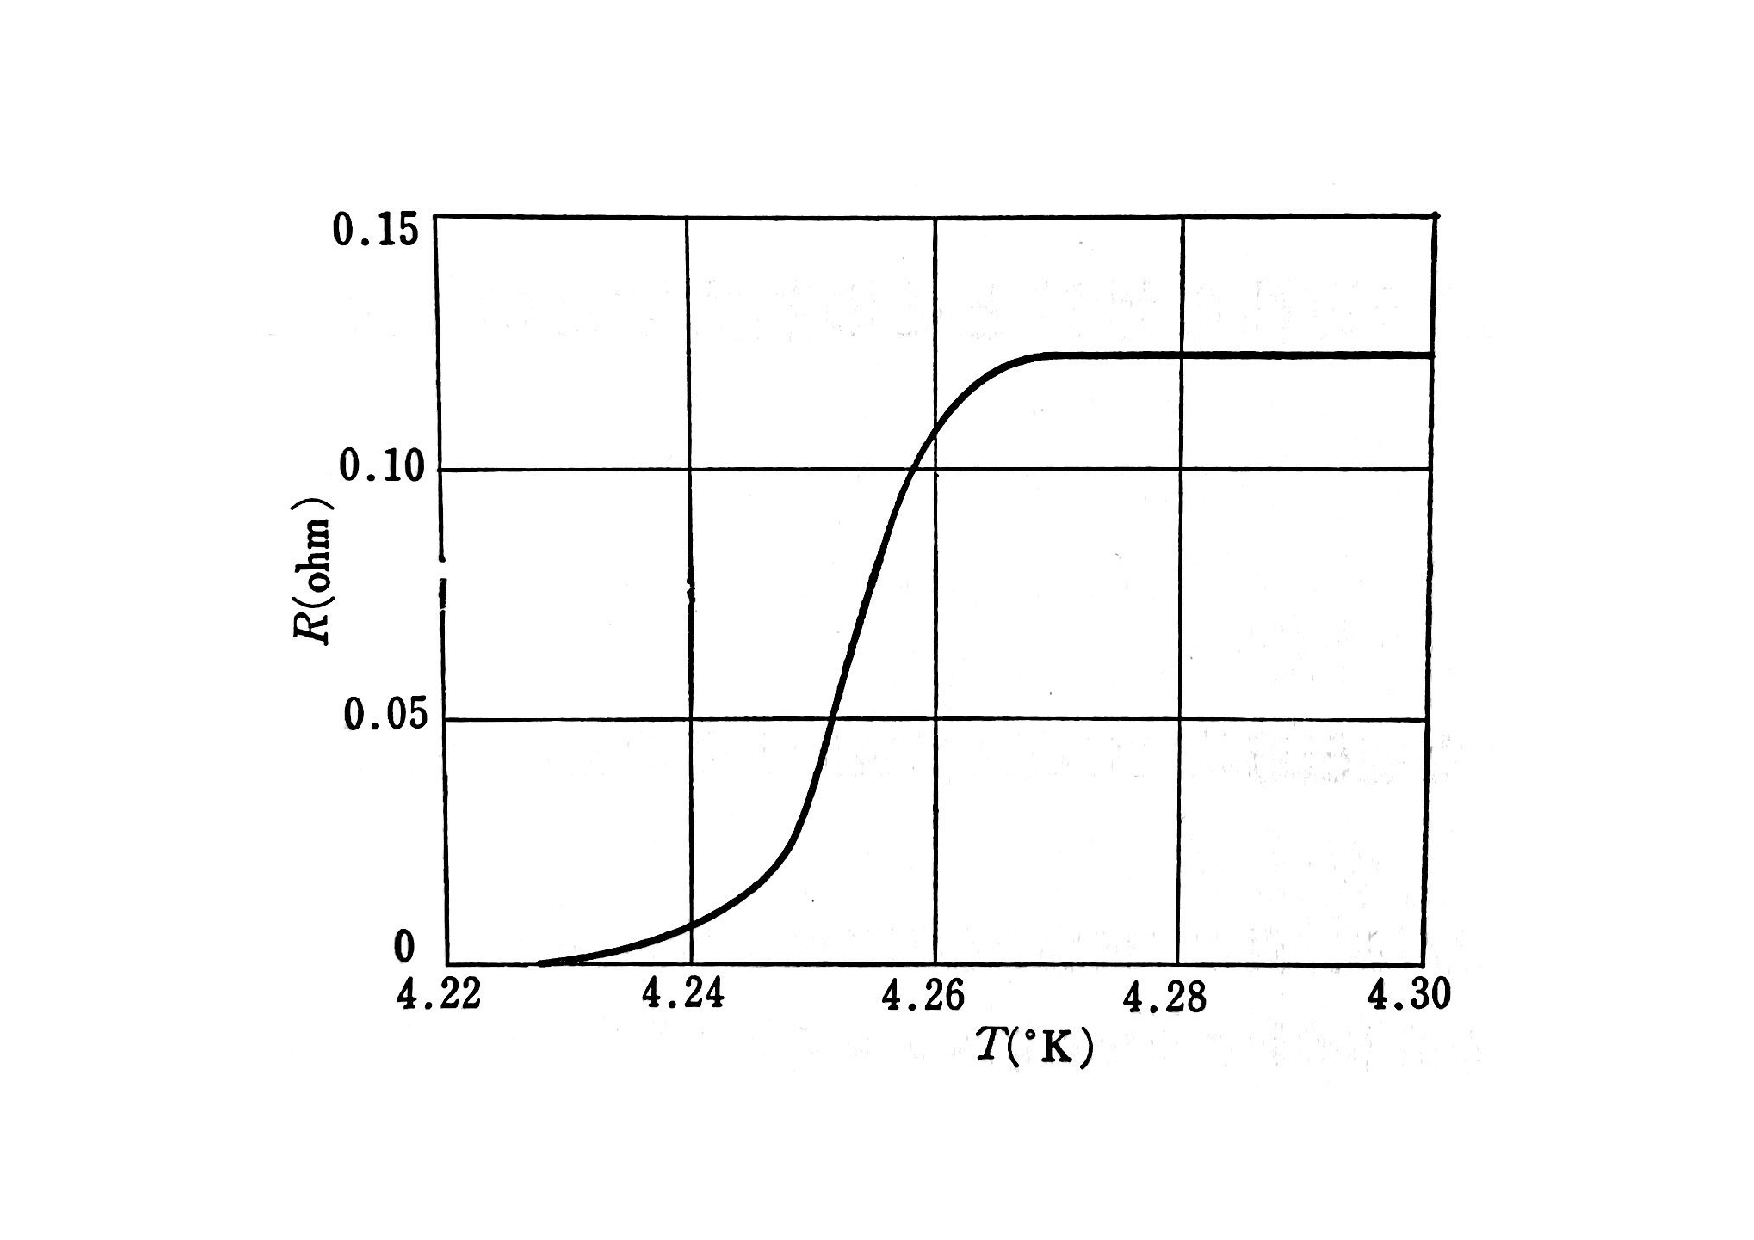
\includegraphics[width=20cm, bb=9 9 900 500]{./section2Proposal/mercury.pdf}
  \caption{Temperature-Resistance relationship on mercury \cite{2_2}.}
  \label{fig:mercury}
\end{figure}

Additionally, Kamerlingh has also found that the superconducting state can be corrupted if imposed by certain magnetic fields of tens of mT. The magnetic field in which a material can tolerate to retain its superconducting state is called the "critical field".
The critical field is often related to the temperature.
In Fig. \ref{fig:H-T}, an example of the critical field - temperature curve is shown.
From which, we can see that most of the conventional metals only have the ability to maintain superconductive under a very low temperature of several Kelvin, and tens of mT of imposed field.
This indicates that the superconducting state is a relatively unique state which only occurs in extreme conditions and can be corrupted easily.
\begin{figure}[H]
  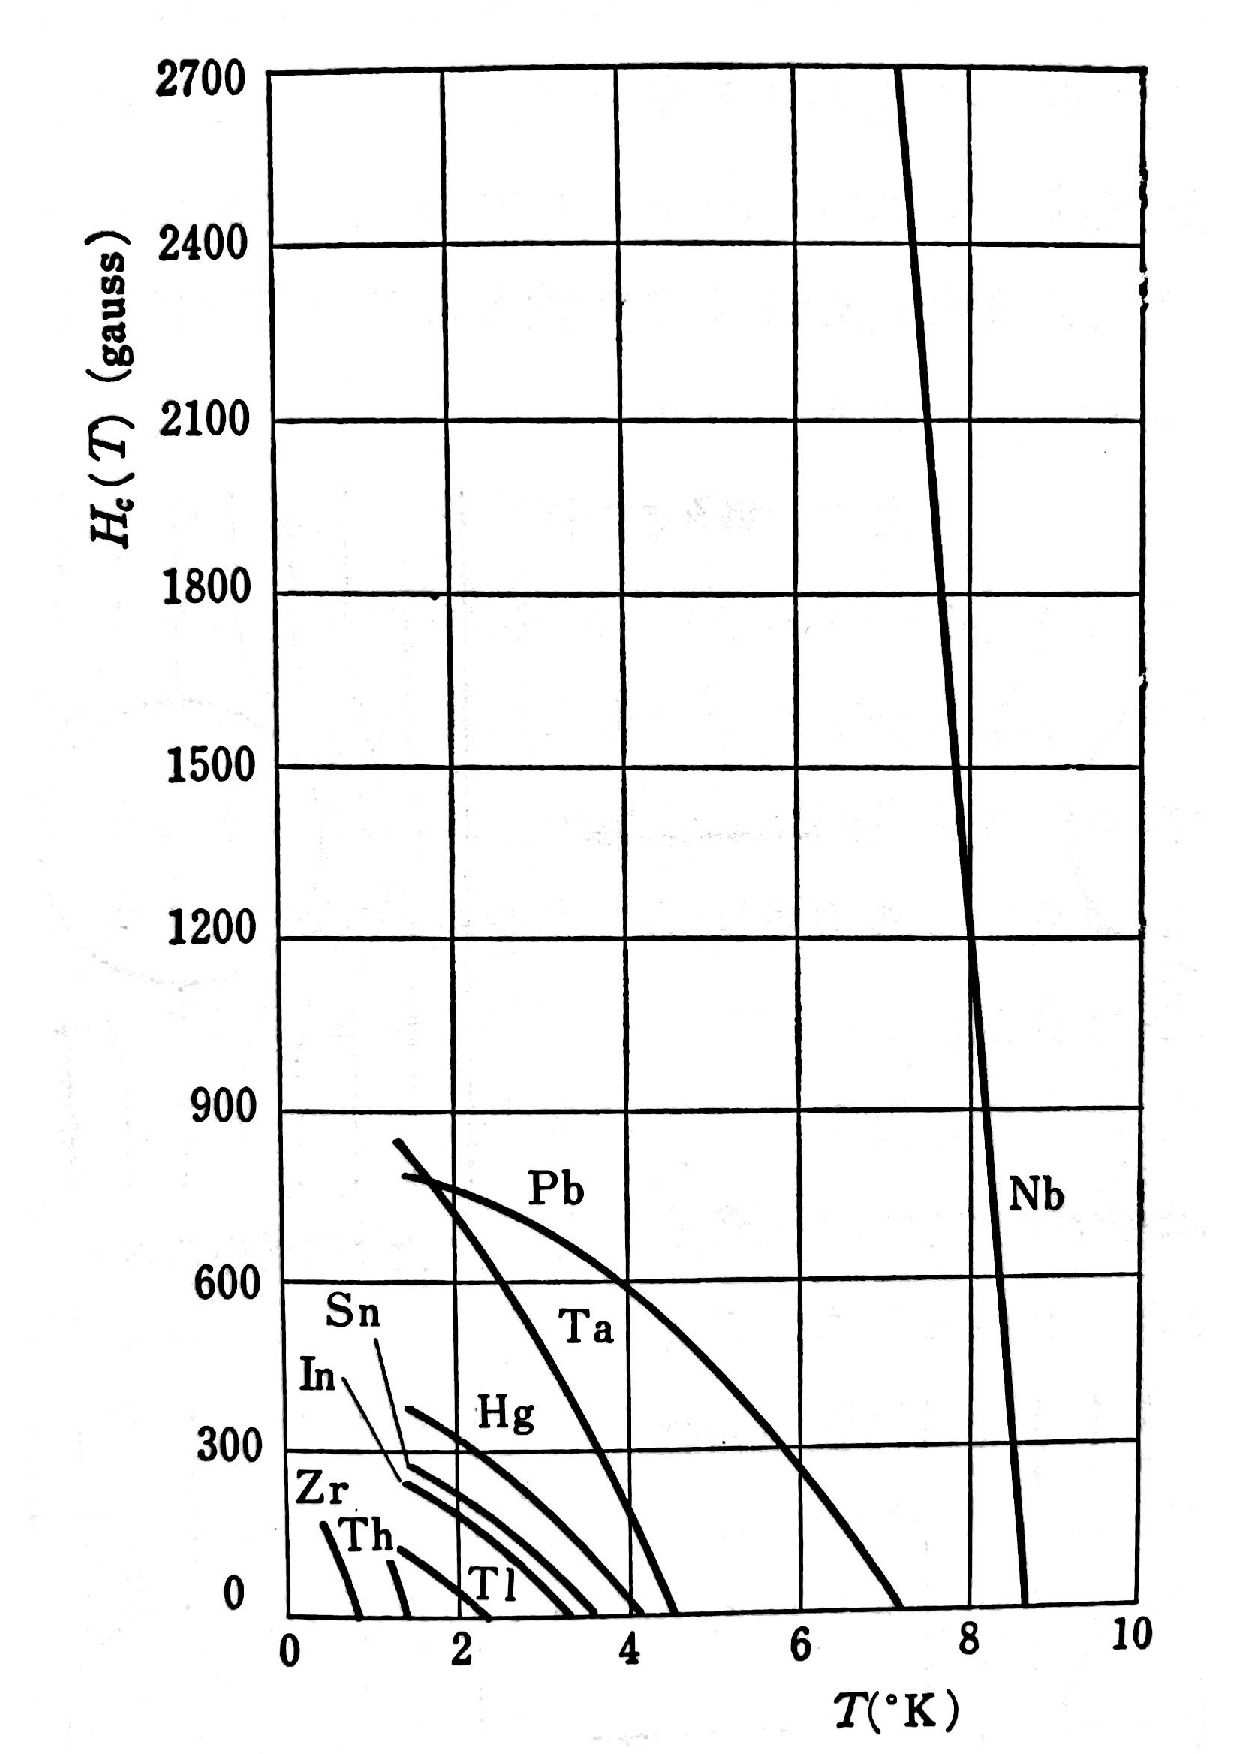
\includegraphics[width=15cm, bb=9 9 900 900]{./section2Proposal/H-T.pdf}
  \caption{Critical Field(H) - Temperature curves observed on several metals \cite{2_3}. Note that 10 Gauss = 1 mT.}
  \label{fig:H-T}
\end{figure}

Note that superconductivity is a special state into which some specific material can transit under certain conditions,
rather than pointing the material itself.
The transition can be concerned as a general phase transition under certain conditions occured in the environment.
To avoid confusion, we tend to use the phrase "superconducting state" instead of "superconductor" in this thesis.


\newpage
\subsubsection{Perfect Conductivity}
The fact that in the superconducting state the electrical resistance drops to an unobservable level has been varified by many experiments \cite{2_4}.
If the zero resistance can be seen as the electrical conductivity $\sigma$ being nearly infinitive,
due to Farraday's rule and ohm's rule,
\begin{eqnarray}
  \mathrm{rot}\bm{E} = \frac{\partial \bm{B}}{\partial t}\\
  \bm{J} = \sigma \bm{E}
\end{eqnarray}
we have
\begin{equation}
  \lim_{\sigma \to \infty} \mathrm{rot} \frac{\bm{J}}{\sigma} = \frac{\partial \bm{B}}{\partial t} = 0
\end{equation}
which indicates that the magnetic field $B$ doesn't change from the initial value in a superconductor.
This scheme can be realized as the "conservation of inital field",
in which the initial field means the field imposed at the exact point of time when the material went into the superconducting state.
An example about this expactation is shown in Fig. \ref{fig:perfectConductivity}.
\begin{figure}[H]
  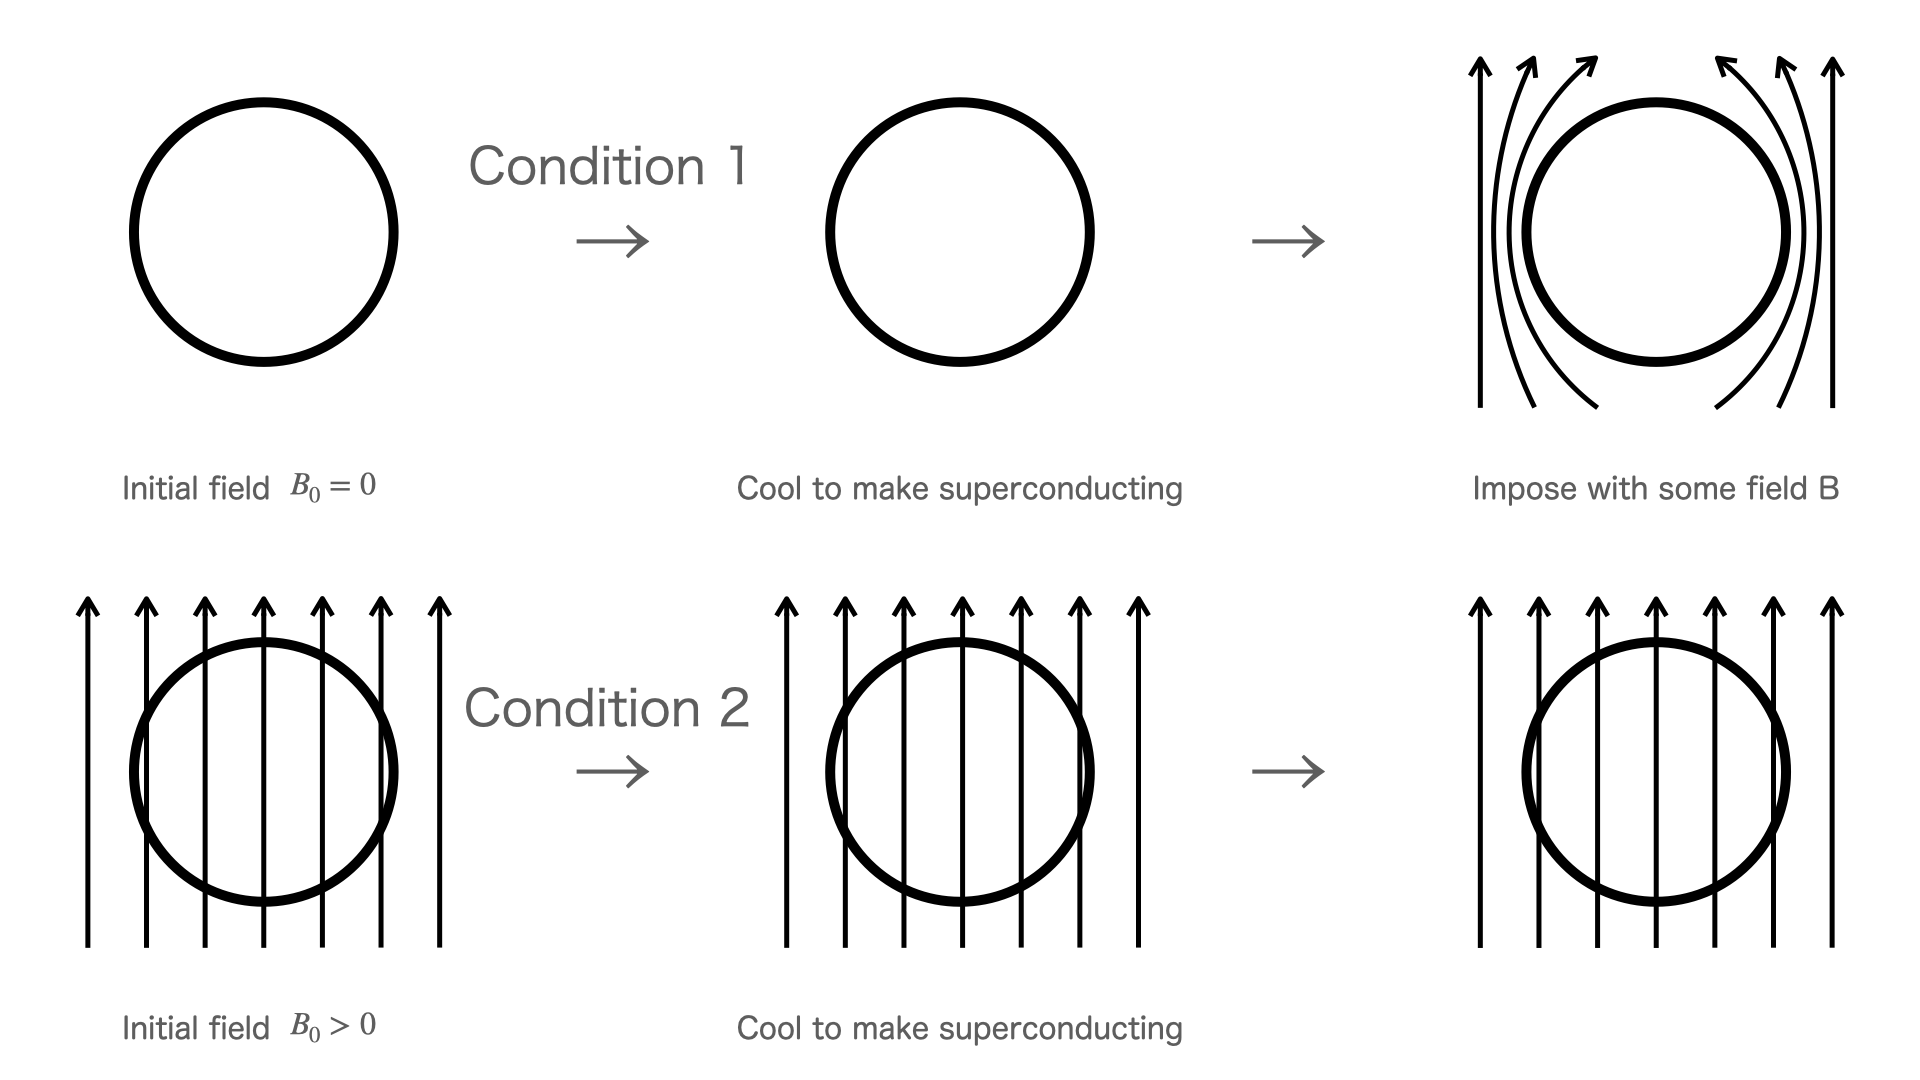
\includegraphics[width=18.5cm, bb=9 9 900 500]{./section2Proposal/perfectConductivity.png}
  \caption{The {\bf expected} magnetic field distribution around a solid ball in the normal state and superconducting state under different initial fields. \cite{2_1}}
  \label{fig:perfectConductivity}
\end{figure}
In condition 1, where the material enters its superconducting state with the initial imposed field $B_0$ being zero,
shows the conservation of zero magnetic flux when it is later imposed with certain $B > 0$.
In condition 2, where the material is first given some initial field $B_0 > 0$ before it becomes superconducting,
again should show the conservation of $B_0$ magnetic flux during all periods.
This expactation is directly derived from the Maxwell equation (3), which explains the behavior of the magnetic field in a perfect conductivity $\sigma \to \infty$ situation.
For a long period this phenomanen was believed to be actually occuring inside a superconducting material,
and many experiments have shown an imitate distribution of Fig. \ref{fig:perfectConductivity}.

If this is true, all of the possible states of the magnetic field distribution inside a superconductor must be thermodynamically balanced,
which is hard to imagine.
Though semi-equilibrium states do exists in reality such as glass at low temperature and overcooled liquid,
in a state where electrons can move without any resistance,
the achievement of such semi-equilibrium situation is difficult to explain.
In fact, instead of fully investigating the mechanism occurs in a superconducting state,
equation (3) $\frac{\partial{\bm B}}{\partial t} = 0$ only describes what would have happened assumed that the conductivity is near infinity.
Also, assurance that the Maxwell equation would hold in such state could not be made before considering the molecular interaction from the perspective of quantum mechanics.


\subsubsection{Meissner Effect (Perfect Diamagnetism)}
Not until the magnetic field distribution near a superconductor measured by Meissner and Ochsenfeld striclty in 1933 has the story changed dramatically \cite{2_5}.
In the experiment focusing on stannum,
they first imposed some parallel field and then cool it into the superconducting state.
In contrast of the expectation shown in Fig. \ref{fig:perfectConductivity},
a significant change on the magnetic field around the material was observed at the transition temperature.
The magnetic flux behaved like being removed from the superconductor,
as the one shown in Fig. \ref{fig:meissner}.
On the surface of the solid superconductor ball,
the vertical component of magnetic field became zero and the field $B$ inside disappeared.
This unexpected result has indicated that
the eigen magnetic behavior in a superconductor is
\begin{equation}
  {\bm B} = 0
\end{equation}
not
\begin{equation}
  \frac{\partial{\bm B}}{\partial t} = 0 \nonumber
\end{equation}
This phenomanen described by equation (4) is called "Meissner Effect",
and is concerned the most original property of a superconductor.
Nowadays, only when a material achieves both zero resistance and the Meissner effect can be declaimed as a superconductor.
\begin{figure}[H]
  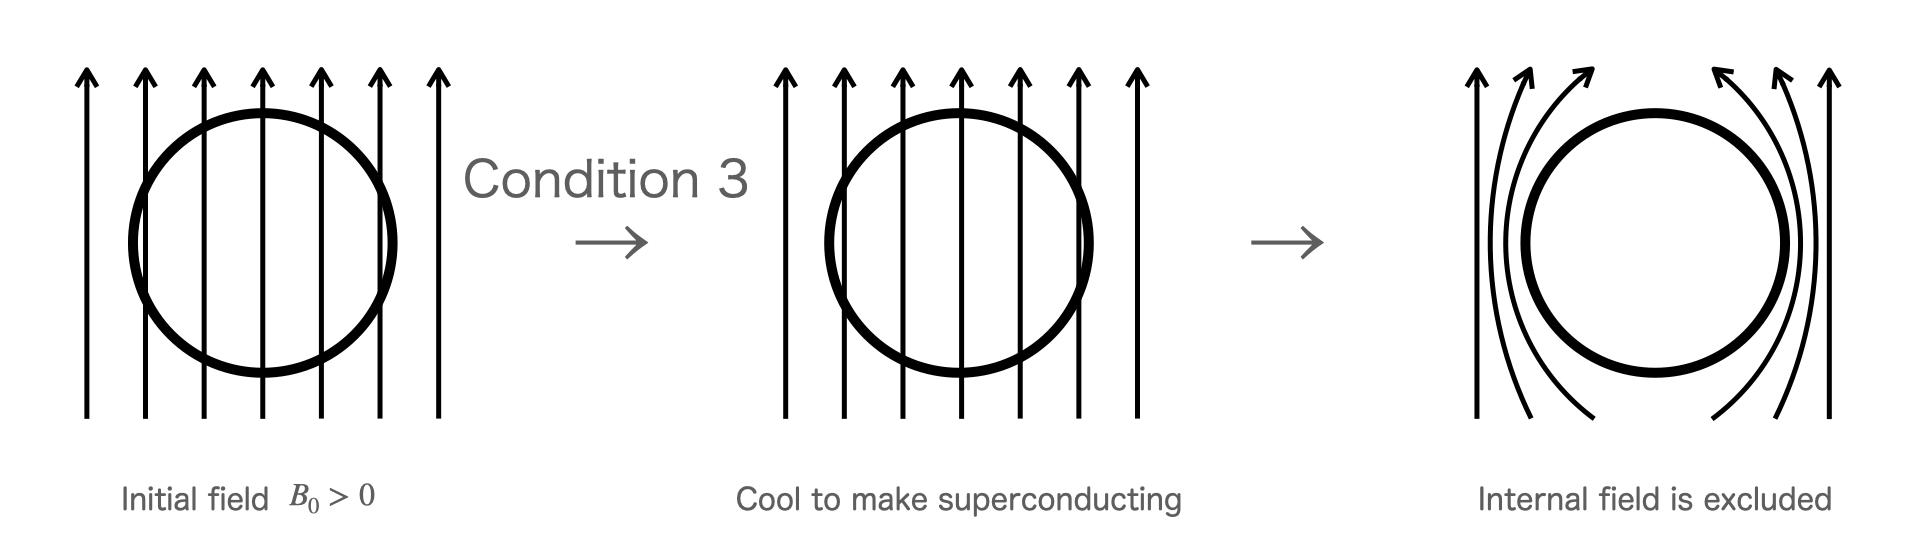
\includegraphics[width=18.5cm, bb=9 9 900 260]{./section2Proposal/meissner.png}
  \caption{The concept of Meissner effect: $B = 0$.}
  \label{fig:meissner}
\end{figure}

Why does it take scientists decades to find this phenomanen?
The Meissner effect could be obscured due to impurities in superconductor or inhomogeneous distribution of the material.
The fact that "frozen" magnetic flux in superconductor under unideal condition is observed
may be considered as the superconducting part and the normal part existing simultaneously in the material.
For instance, if the crystal of the metal is inhomogeneous, then in the superconducting state, the inhomogeneous part may distort the nearby field.
If the magnetic field density is somehow high in certain region,
the superconducting state may collapse partially,
turning the crystal into a state mixed by superconducting and normal regions.
Theese pratical conditions make the magnetic flux "locked in" some normal parts in a superconductor.

To continue, whether a normal region can exist in the superconducting state is the key difference between the so called first kind and second kind superconductor.
In an ideal (pure and homogeneous) metal, such as mercury and those been tested by Kamerlingh (see Fig. \ref{fig:H-T}),
magnetic flux is unable to penetrate it during the superconducting state due to the Meissner effect.
Consequently, theese crystals, known as the first kind of superconductor,
usually have a low critical field and a low transition temperature,
since their tolerance to external turbulence on electromagnetic and thermodynamic is poor.
In contrast, superconductors consists of complicated compounds such as CuO2 and those labeled as the High Temperature Superconductor
allow the normal region to emerge during the superconducting state.
Theese compounds, named the second kind of superconductor,
do not show the perfect Meissner effect but are capable to tolerate a much more higher field and temperature.


\newpage
\subsection{High Temperature Superconductor(HTS) Tape}
Great imporvements had been achieved these years on manufactoring superconductor having a high critical current and transition temperature.
Generally, the conventional superconductors discovered in the 1910s usually are well-known pure metals and only transit to the superconducting state in an extremely low temperature of a few Kelvins.
In 1986, J. G. Bednorz and K. A. Müller has found that superconductivity transition has occured at 30 K in the copper oxide Ba-La-Ci-O compound.
In the next few years, superconductors with transition temperature above the boiling point of nitrogen, 77 K,
are discovered in copper oxide crystals,
which allows the generation of the superconductivity more easily using liquid nitrogen.
Copper based superconductors had long been the state-of-the-art high temperature superconductor having a high transition temperature and a pratical manufactor process.
Dosens of studies had been conducted on them, until a break through on the transition temperature was made by hydrogen sulfide under extremely high pressure of 100G Pa \cite{2_8}.
In late 2020, Snider et al. has marked an record of achieving a superconductivity transition at room temperature ($14^\circ \mathrm{C}$) \cite{2_9}.
The whole timeline of the high temperature superconductor development is shown in Fig. \ref{fig:HTSs}.
\begin{figure}[H]
  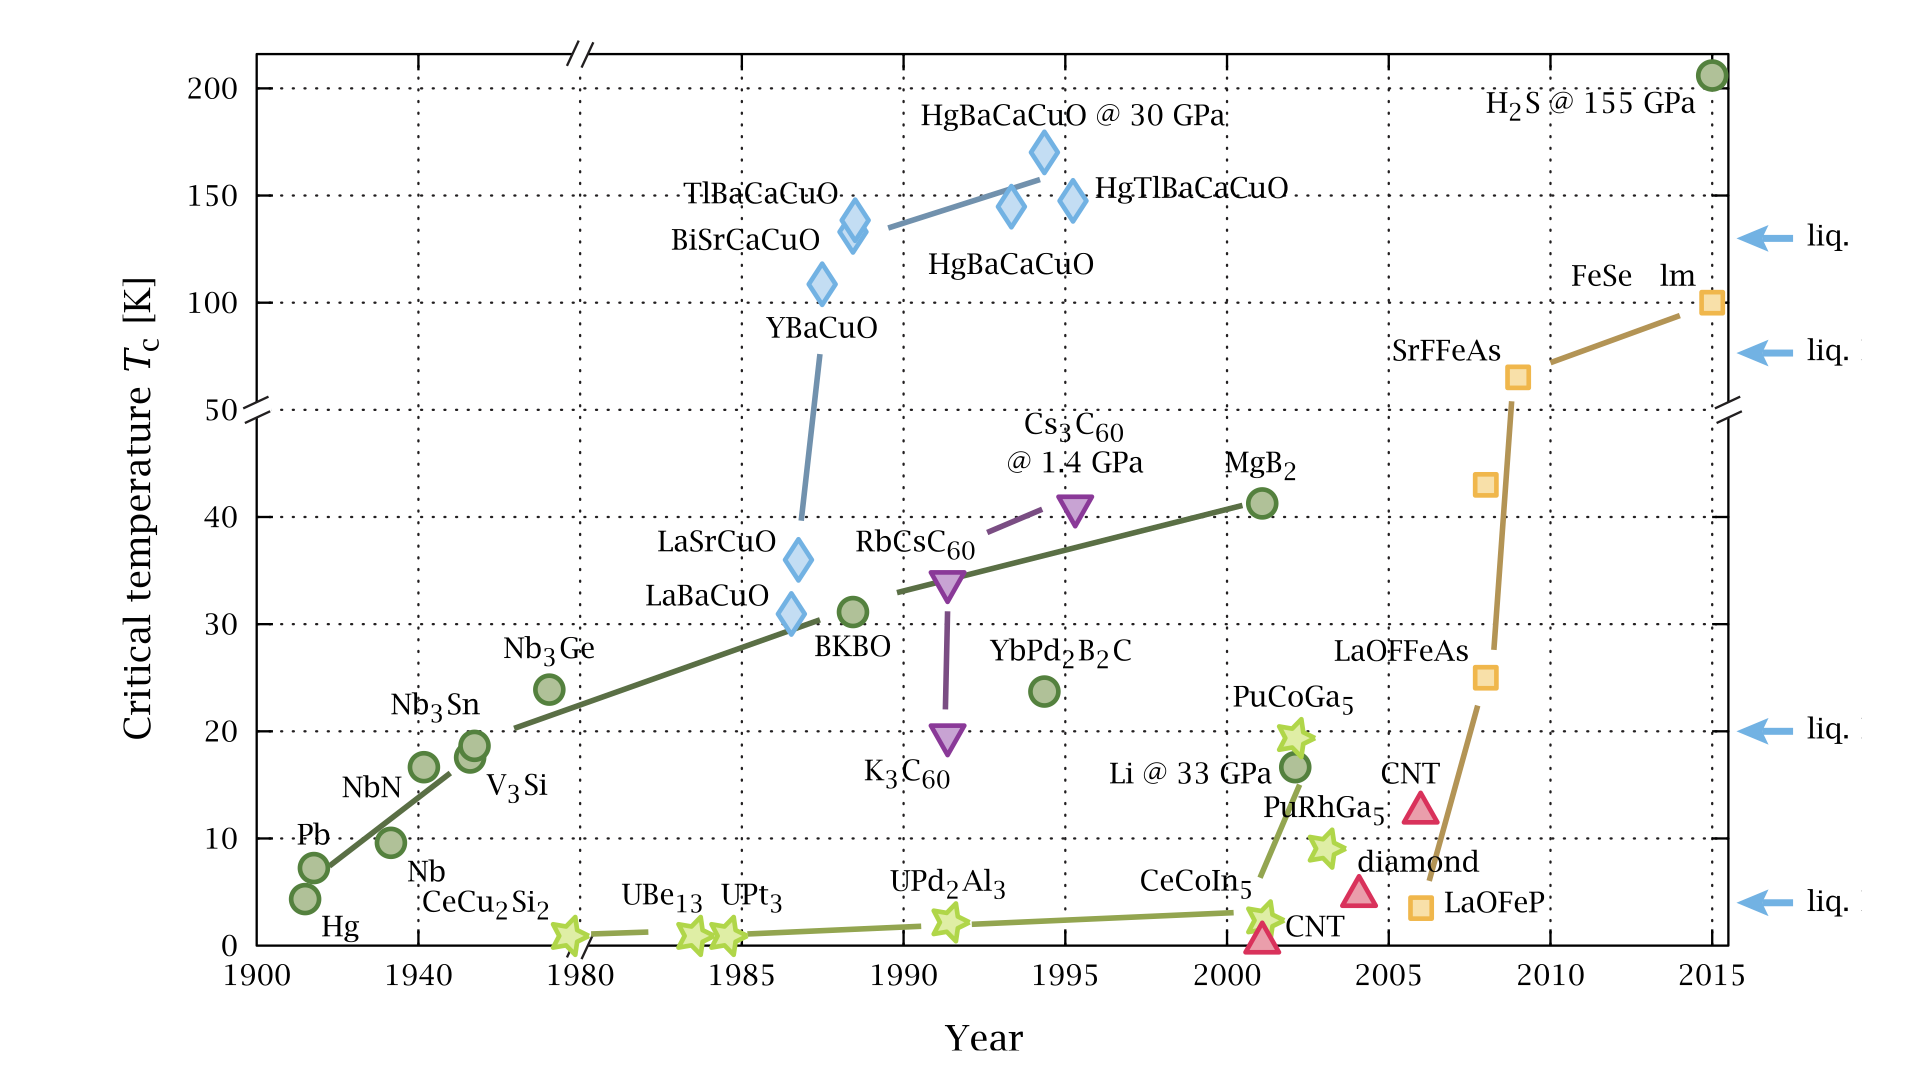
\includegraphics[width=18.5cm, bb=9 9 900 500]{./section2Proposal/HTSs.png}
  \caption{}
  \label{fig:HTSs}
\end{figure}

To avoid confusion, theese superconductors discovered after 1980s which have higher transition temperatures, tolerable on higher currents,
allow magnetic field penetration (which makes them the second kind superconductor in classification),
are often called the High Temperature Superconductor(HTS).
The superconductors discovered before then,
which have lower transition temperatures, show an ideal Meissner effect, classified into the first kind superconductor, are often called the Low Temperature Superconductor.

In our study, we use the copper oxide superconductor YBa2Cu3O7(YBCO) due to its stable supply and the availability with liquid nitrogen cooling.
The YBCO superconductor is generally manufactored in a tape form, within which electrons is able to move without resistance along the long axis.
At the production level, a pure copper or silver layer is often additionally overlaid to increase electrical stability.
The structure of the whole tape is shown in Fig. \ref{fig:Y},
and the specification of the superconductor used through this thesis is shown in Tab. \ref{tab:Y}.
\begin{figure}[H]
  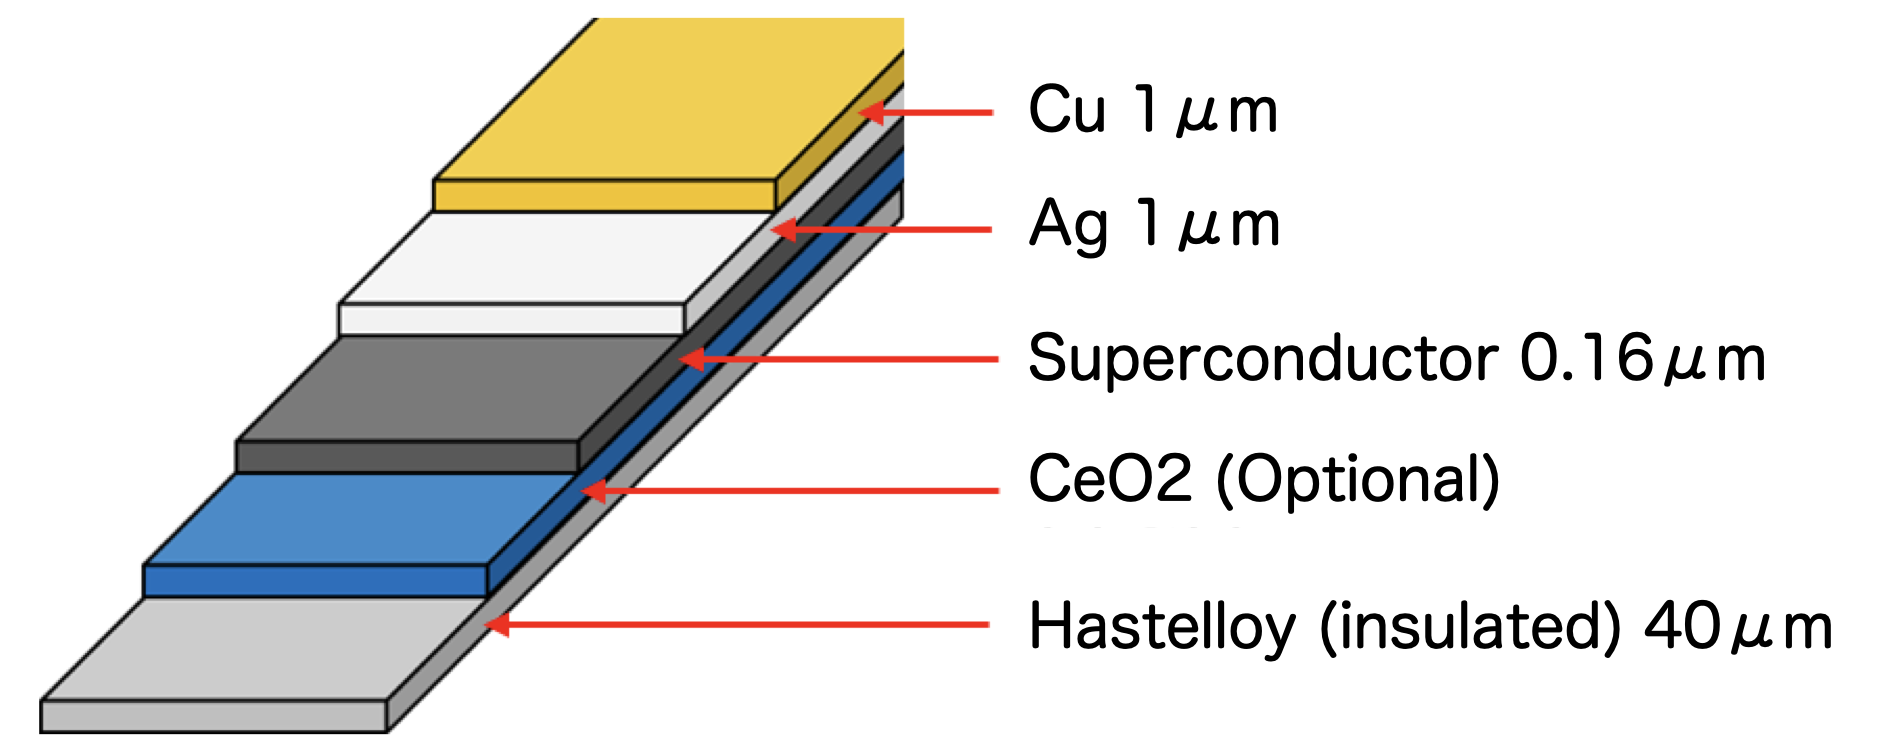
\includegraphics[width=18.5cm, bb=9 9 900 360]{./section2Proposal/Y.png}
  \caption{The layers of a conventional high temperature superconductor tape.}
  \label{fig:Y}
\end{figure}
\begin{table}[H]
  \centering
  \caption{Shielding effects under various magnet thickness(a/b) and relative permeability($\mu_r$).}
  \label{tab:Y}
  \begin{tabular}{cc|rrrrr}\hline\hline
    a/b &  & 0.99 & 0.8 & 0.6 & 0.4 & 0.2\\\hline
    $H_{internal}/H_{external}$ & $\mu_r = 100$ & 3/5 & 1/12 & 1/18 & 1/22 & 1/23 \\
    $H_{internal}/H_{external}$ & $\mu_r = 1000$ & 3/23 & 1/109 & 1/175 & 1/209 & 1/221 \\\hline\hline
  \end{tabular}
\end{table}

The question why many materials show the mysterious behavior of superconductivity remains open, although a part of it is considered solved.
In 1948 Fritz London proposed that the phenomanen may be consequences of the coherence of a quantum state \cite{2_10}.
With further studies, a widely accepted explanation has been published by J. Bardeen, L. Cooper and J. R. Schrieffer in 1957, called the BCS theory \cite{2_11}.
Generally, it was considered impossible for electrons to move without resistance above strict 0 K since the atom vibration was assumed unavoidable from a thermodynamic perspective.
To reach the state of superconductivity, some attractive forces must have worked to condensate electrons into groups which have the state of minimum energy.
However, since the electron is a fermion, the Pauli exclusion principle and the Coulomb repulsion must be overcame before it can be condensated.
The BCS theory assume that electrons attracted each others by exchanging the phonon, and consequently bound together in Copper pair forms in which the state has a lower energy than the Fermi energy.
This minimum energy state achieved by Copper pair origined from the electron-phonon interaction is believed to be the cause of the conventional superconductivity.
While this theory can explained most of the superconductor found before 1980s, namely the first kind superconductor or the low temperature superconductor,
it fails to give a full derivation on the modern high temperature superconductor.

For the HTS, the formation of Copper pair is considered to be somehow participated in the mechanism, but agreement on the reason hasn't been reached.
A relatively new theory has been published in 2016 \cite{2_12}, claiming that an unexplained behavior of the electrons in HTS,
which might be the direct origin of superconductor, has been observed in computer simulation.
Denoting the full detail of the mechanism in superconductivity is beyond the scope of this thesis,
but the phenomanen can be realised in a macroscopic perspective from which the perfect conductivity can be achieved and the notable Meissner effect should be marked.
A well written macroscopic introduction of superconductivity by Fritz London is available in his book \cite{2_10}.


\newpage
\subsection{Ferromagnetism}
\subsubsection{Sense of Magnetism}
Before the ferromagnetism is discussed, we would like to introduce some important properties of magnetism which even undergraduated students majored in electrical engineering might not have learned deeply.
To know the fundamental of a magnetic field, first we tried to measure the magnetic force among various materials.
Consider a huge coil which generates a 3 T field in the central point, like Fig. \ref{fig:2_coil}.
\begin{figure}[H]
  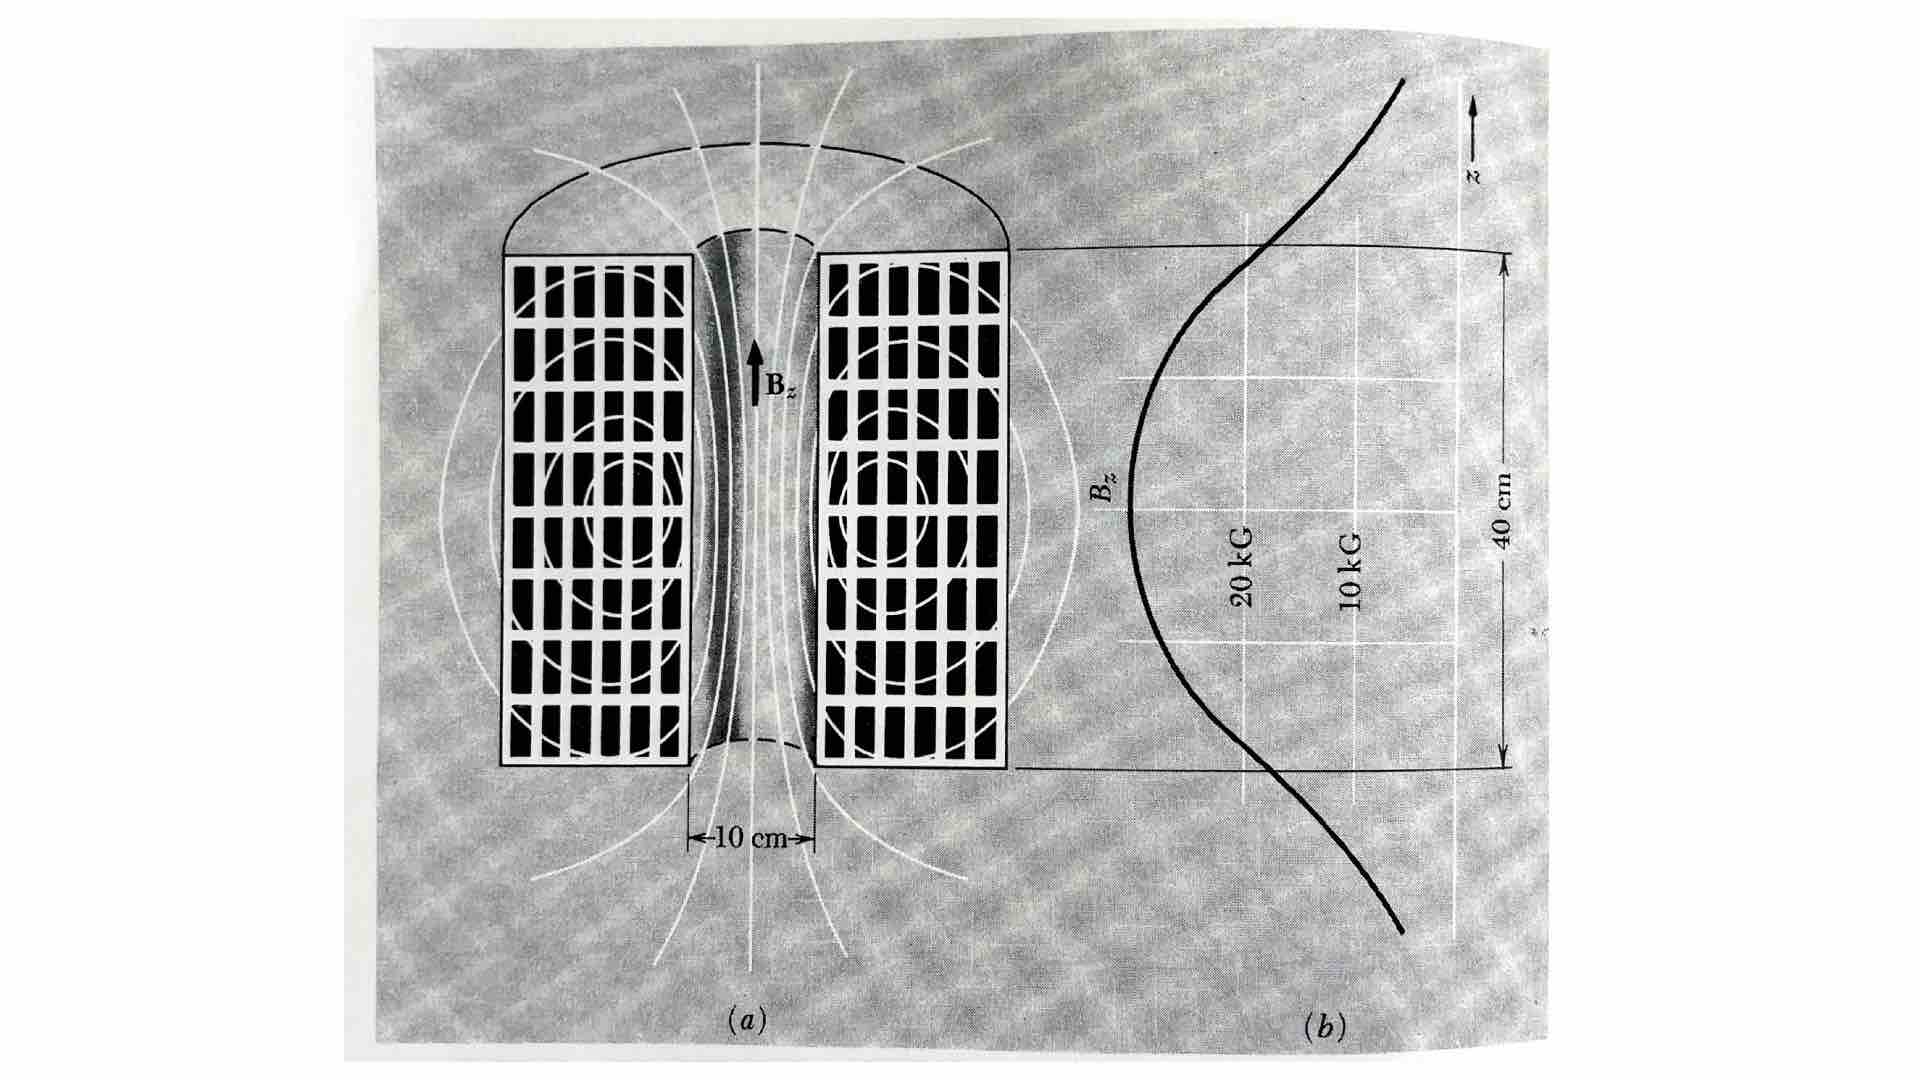
\includegraphics[width=18.5cm, bb=9 9 900 500]{./section2Proposal/3TCoil.JPEG}
  \caption{Schematic drawing of a conventional coil.\cite{2_13}}
  \label{fig:2_coil}
\end{figure}
The field is $10^5$ times of the geomagnetism, and is approximately 10 times more than the field near a common magnet.
From which, we know that the coil used in our experiment is a relatively large scale but not completely unrealistic one at all.
If we measured the force exerted on different materials when they are put along the central axis of the coil,
we would get some interesting results:
\begin{table}[H]
  \centering
  \caption{Force recieved in the electric coil among different materials.\cite{2_13}}
  \label{tab:2_coilResult}
  \begin{tabular}{cr}\hline\hline
    Material & Force [mN] (positive for attraction) \\\hline
    Diamagnetic & \\
    $\mathrm{H_2O}$ & $-2.2$\\
    Cu & $-0.26$\\
    NaCl & $-1.5$\\
    S & $-1.6$\\
    C (graphite) & $-1.6$\\
    C (diamond) & $-11.0$\\
    $\mathrm{N_2}$ (liquid@78 K) & $-1.0$\\\hline
    Paramagnetic & \\
    Na & $+2.0$\\
    Al & $+1.7$\\
    $\mathrm{CuCl_2}$ & $+28.0$\\
    $\mathrm{NiSO_4}$ & $+83.0$\\
    $\mathrm{O_2}$ (liquid@90 K) & $+750.0$\\\hline
    Ferromagnetic & \\
    Fe & $+40,000$\\
    $\mathrm{Fe_3O_4}$ & $+12,000$\\\hline
  \end{tabular}
\end{table}
\begin{enumerate}
  \item The maximum force occured not at the central point, but where the $dB_z/dz$ maximized, namely at the edge of the coil.
  \item The exerted force is related rather to the weight than to the shape of the sample .
  \item Despite the powerful field we have prepared, for most of the samples, the force measured is way too small.
  For typical values, $0.1\sim0.2$ N/kg are measured, which is no greater than a few percentage of their weights.
  \item When the imposed field is increased continueously, some samples tend to be attracted while the others are repulsed.
  This completely opposite behavior against magnetic force among the samples are extraordinary,
  and immediately indicates that the common materials on Earth can be devided into 2 groups,
  one attracted by the magnetic field, the other being repulsed.
  \item Within the samples, we have discovered a few of them showing strong attraction from the field.
  For example, the crystal of $\mathrm{CuCl_2}$ is attracted by $2.8$ N/kg down into the central.
  Liquid oxygen has shown an attraction of $75$ N/kg, about 8 times larger than its weight.
  On contrast, liquid nitrogen only showed a weak repulsion of $10^{-4}$ N/kg.
  The same trend occured on copper and iron, among which a huge difference of $10^5$ N in magnitude is observed.
  The total result is stated in Tab. \ref{tab:2_coilResult}.
  \item Whether the force changed proportionally to the imposed field has also shown an obvious difference between the samples.
  When the imposed field was cut in a half,
  forces measured on the materials listed before iron in Tab. \ref{tab:2_coilResult} descreased to $1/4$,
  while the others only dropped to about $1/2$ or even higher.
\end{enumerate}

From the above, obviously, the phenomanen we are facing is complicated.
For the first step to understand magnetism, some classification should be introduced.
Materials showing weak repulsion on magnetic fields are called "diamagnetic",
which most of the materials on Earth are listed in, except for a few inorganic compounds \cite{2_13}.
Diamagnetism is considered a consequence of the general electromagnetic induction from the electron.
Consider a ring made of conductive ingredients.
If it is pushed towards a magnetic field penetraing the cross section, electrical current would be induced,
generating an opposite field to push itself outside the field.
This phenomanen, often known as the Lentz's law,
is similar to what has happened in the experiment when we tried to push a material into some magnetic field.
Since every atom contains electrons, diamagnetism is the general behavior when a certain material interacts with the magnetic field.

When attraction on magnetic fields is observed,
it indicates that some other effects more dominant than the diamagnetism must have been participated in.


\newpage
\subsubsection{Modern Ferromagnetic Materials}
Conventional ferromagnets list up ferite, cobalt etc. which hold a relative permeability of 1000-10000 and a maximum magnetization of about 700 mT.
Recent researches have reached a magnetization as high as 1-2 T, using stainless steel and permalloy (a nickel–iron alloy).
The list is shown in Fig. \ref{fig:magnetMaterials}
\begin{figure}[H]
  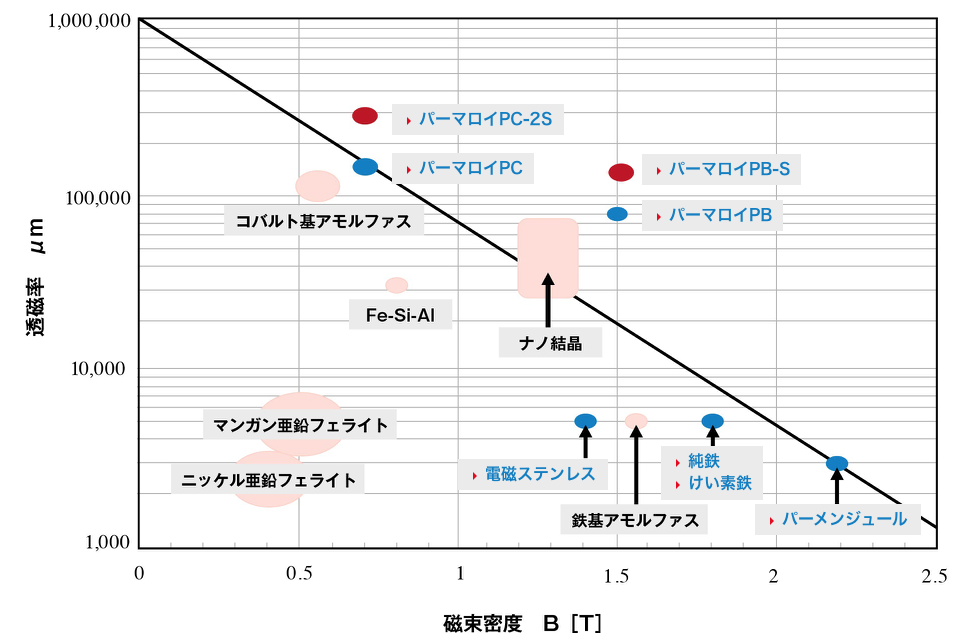
\includegraphics[width=18cm, bb=9 9 900 600]{./section2Proposal/magnetMaterials.png}
  \caption{The conventional and modern ferromagnet materials.}
  \label{fig:magnetMaterials}
\end{figure}
In our research, we have focused on ferite which is a non-oriented ferromagnet with relatively lower maximum magnetization to satisfy our request of simulating a situation in which magnets would go saturated.


\newpage
\subsubsection{Significant but not Apparent Difference among the ${\bm B}$ Field, ${\bm H}$ Field and ${\bm M}$ Field}
In applied electrical engineering, the field $H$ and field $B$ are often seen having the same direction.
This is true in the case that magnetization is not participated in,
while near a strong magnet the magnetization enrolls,
leaving the familiar equation
\begin{equation}
  \mathbf{B} = \mu_0\left( \mathbf{H} + \mathbf{M} \right)\nonumber
\end{equation}

To make it clear, a schematic drawing of the surrounding $B$ and $H$ fields near a magnet is shown in Fig. \ref{fig:BandH}.
\begin{figure}[H]
  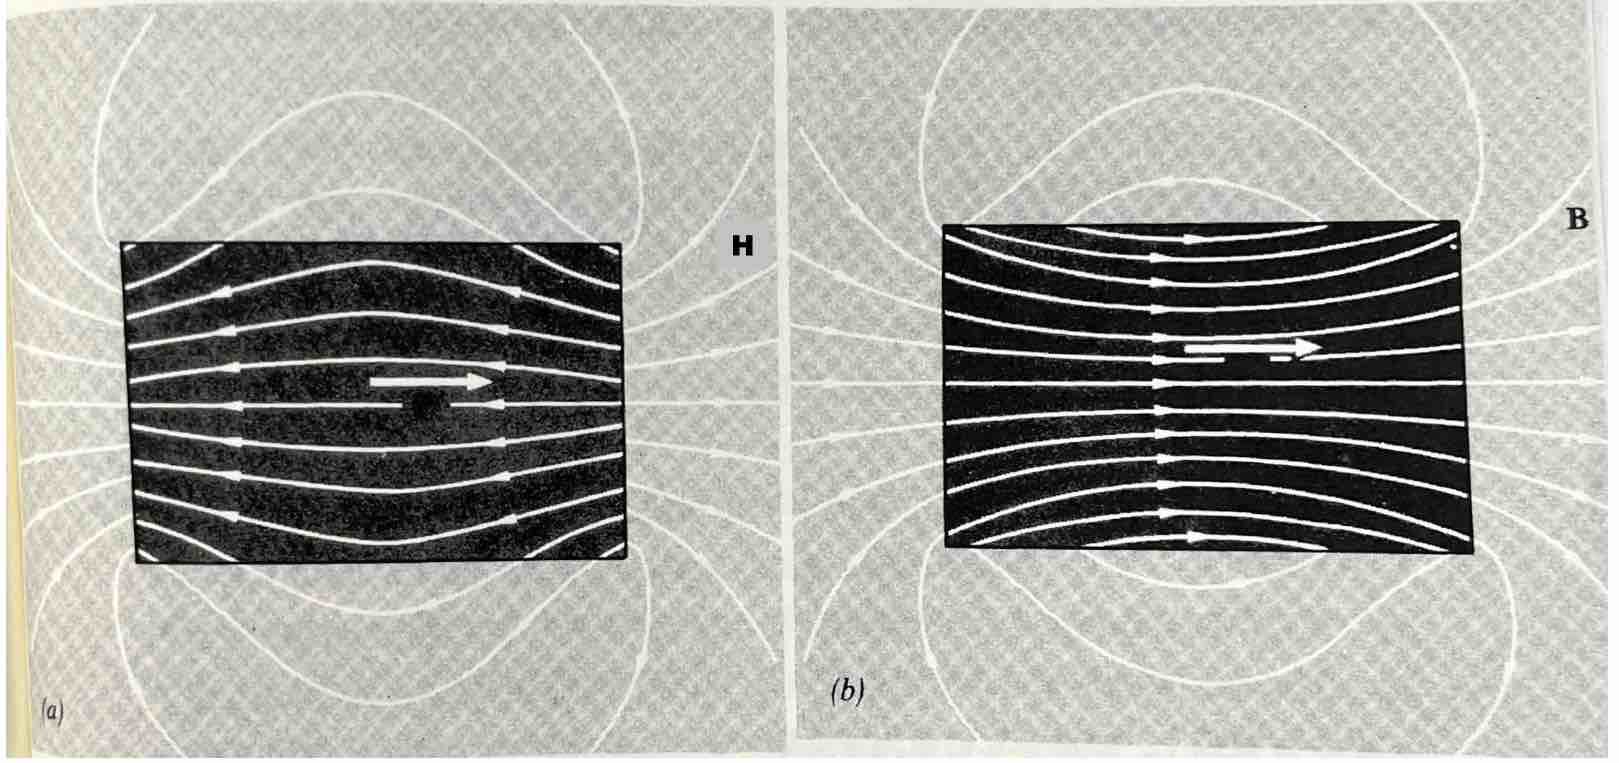
\includegraphics[width=18cm, bb=9 9 900 550]{./section2Proposal/BandH.JPEG}
  \caption{The (left) $H$ field and (right) $B$ field near a conventional magnet.}
  \label{fig:BandH}
\end{figure}
In Fig. \ref{fig:BandH}, it is appearant that both fields on the outside of the magnet distributed identically strictly,
while on the inside part the are totally different with approximately opposite direction.
In fact, the $H$ field is strictly the same as the $E$ field under the condition that the magnet is substituded by a conventional capacitor where opposite irons gathering around the 2 poles.
This indicates that $H$ field can be seen as origining from a scalar potential,
with virtual plus magnetic monopole gathering on the left pole of the magnet,
and minus magnetic monopole gathering on the right pole of it.

The different distribution between the internal $H$ and $B$ field results from the fact that
the $B$ field origins from a vector potential,
or in other terms,
satisfies the equation.
\begin{equation}
  div\mathbf{B} = 0\nonumber
\end{equation}
This equation describes the $B$ field must be continueous anywhere,
generating a near field shown in Fig. \ref{fig:BandH}.

Now, the magnetization term $M$ comes in to fullfill the equation
\begin{equation}
  \mathbf{B} = \mu_0\left( \mathbf{H} + \mathbf{M} \right)\nonumber
\end{equation}
In a magnet, strong $M$ would be exited along the $B$ field to cancel out the $H$ field.
A scematic drawing of this concept is shown in Fig. \ref{fig:BandHandM}.
\begin{figure}[H]
  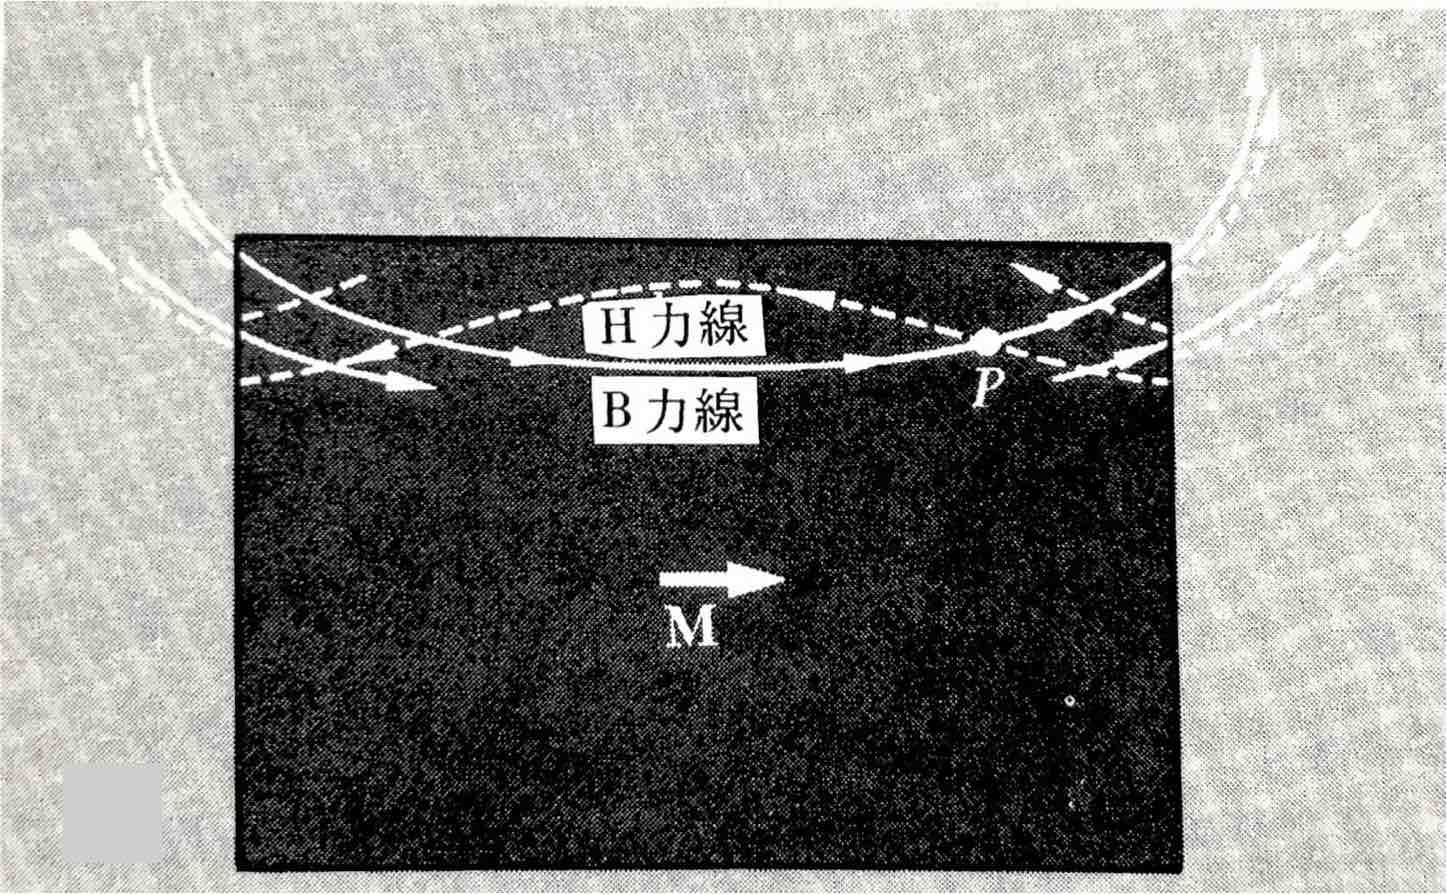
\includegraphics[width=18cm, bb=9 9 900 550]{./section2Proposal/BandHandM.JPEG}
  \caption{The $H$ and $B$ and $M$ field near a conventional magnet.}
  \label{fig:BandHandM}
\end{figure}


\newpage
\subsection{Conventional Magnetic Cloak}
A magnetic cloak using low temperature superconductor bulks and ferromagnets is first published in Fedor's work \cite{2_20}.
The key idea is to combine superconductor bulk with ferromagnet to achieve the cloaking ability,
of which the schematic drawing has been already shown in Fig. \ref{fig:cloak}.
To describe the cloak of magnetic field, the field along certain tangent line on the surface is shown in Fig. \ref{fig:cloakSurfaceLine}.
\begin{figure}[H]
  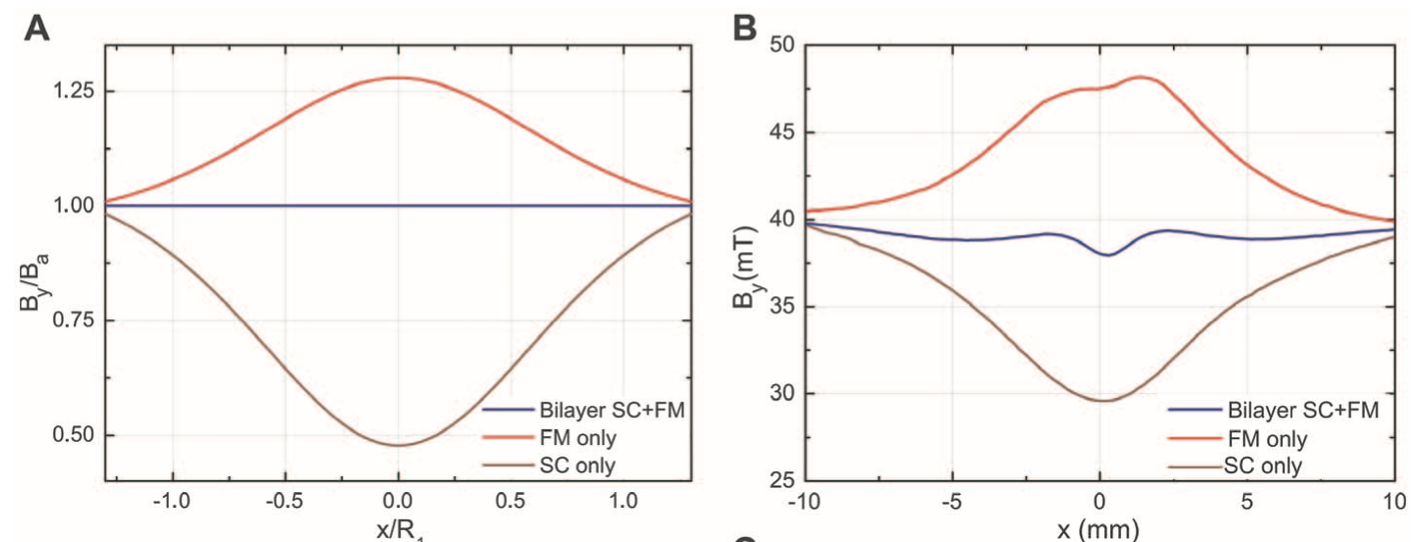
\includegraphics[width=17cm, bb=9 9 900 550]{./section2Proposal/cloakSurfaceLine.png}
  \caption{The magnetic field along the top line. (A) calculation; (B) experimental.\cite{2_20}}
  \label{fig:cloakSurfaceLine}
\end{figure}
From Fig. \ref{fig:cloakSurfaceLine}, it is obvious that nearly perfect cloaking ability can be achieved.
In other words, by adapting the Meissner effect of superconductor and the magnetization phenomenen of ferromagnet,
shielding outer field while not disturbing it is possible.
However, the Meissner effect can only tolerate a few tens of 10 mT, which in turn makes the conventional magnetic cloak impossible to work under high fields.


\subsection{Electromagnetic-Induction Type Magnetic Cloak}
To overcome this problem and develope a magnetic cloak like equipment suit for operation under high fields of a few Tesla,
we have proposed a brand new magnetic cloak named the "Electromagnetic Induction Type Magnetic Cloak",
which applys the perfect conductivity property instead of the Meissner effect.
The main structure is shown in Fig. \ref{fig:EIMCStructure}.
\begin{figure}[H]
  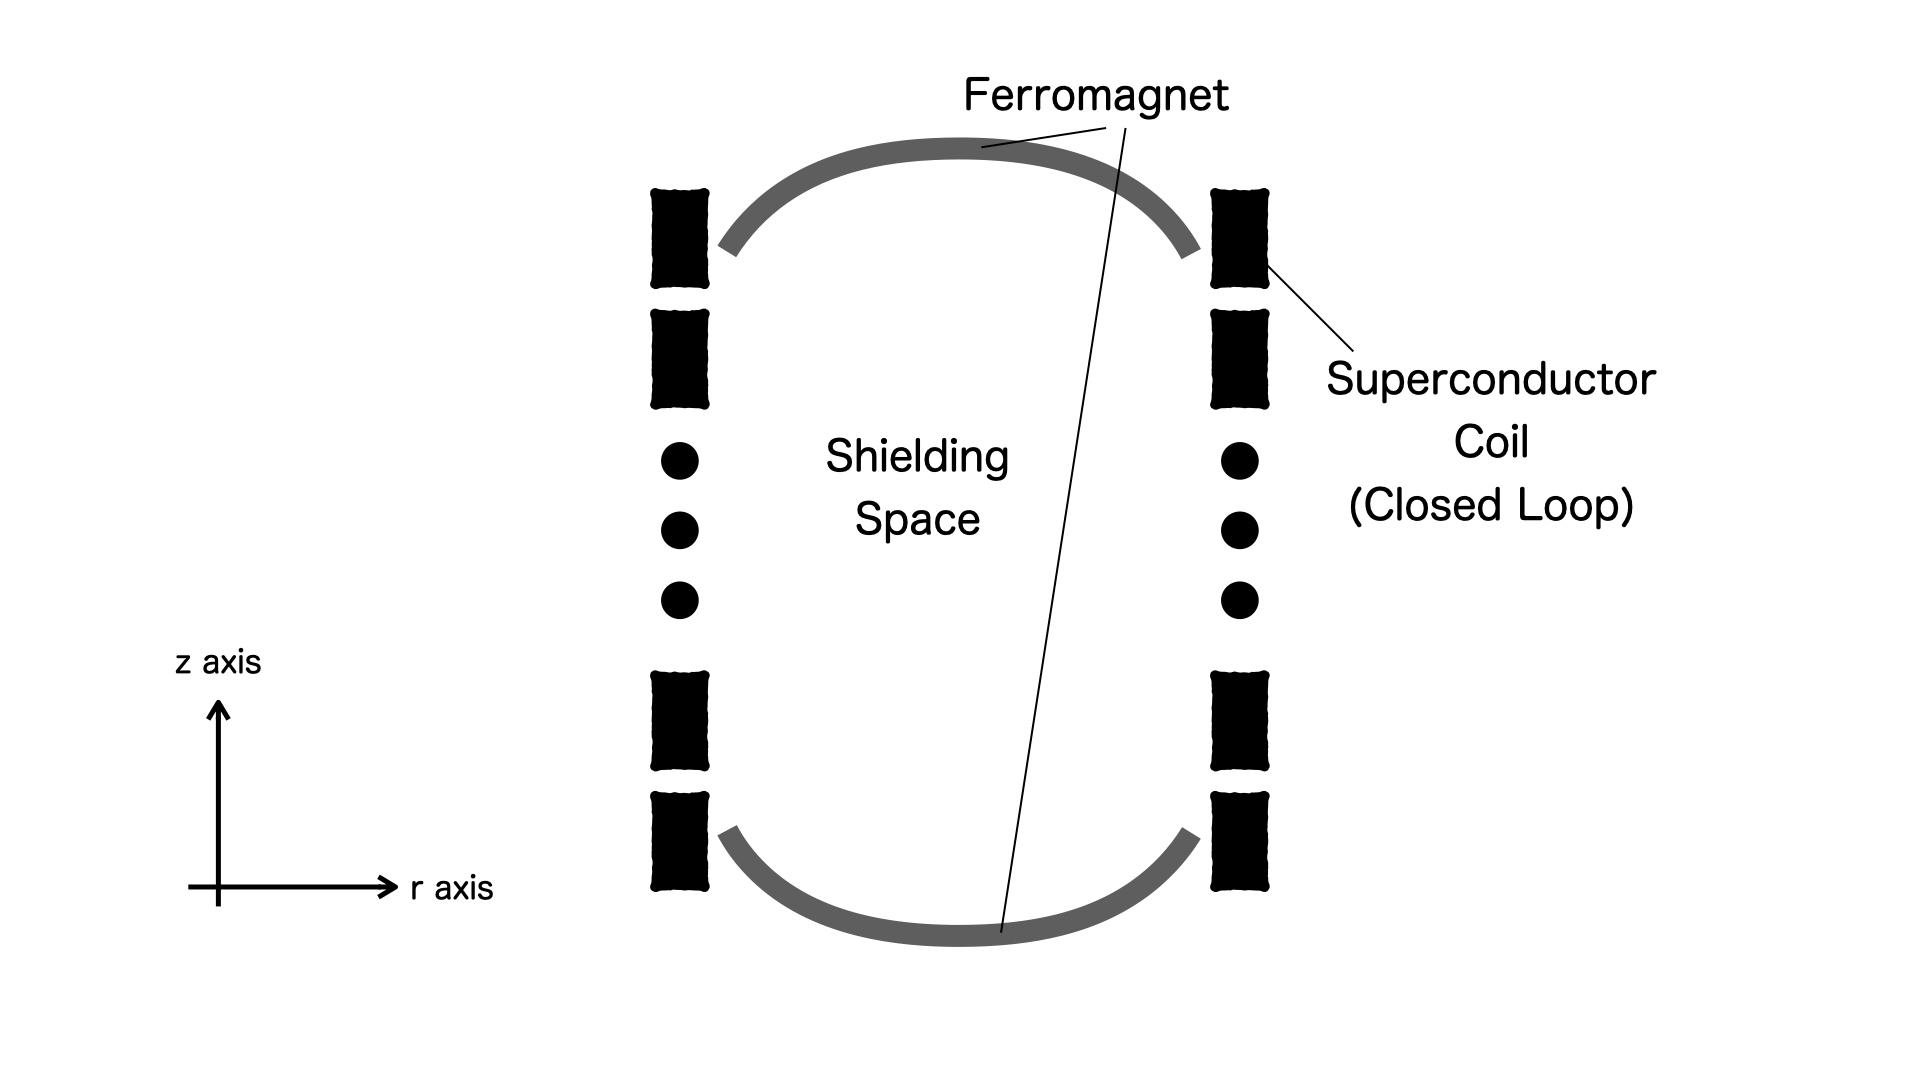
\includegraphics[width=13cm, bb=9 9 900 550]{./section2Proposal/EMICStructure.png}
  \caption{The structure of Electromagnetic Induction Type Magnetic Cloak.}
  \label{fig:EIMCStructure}
\end{figure}
First we connect the superconductor windings to make a huge closed loop.
Then, ferromagnets are placed on the top and the bottom edge of the coil.
The following procedure shows how it works.
\begin{figure}[H]
  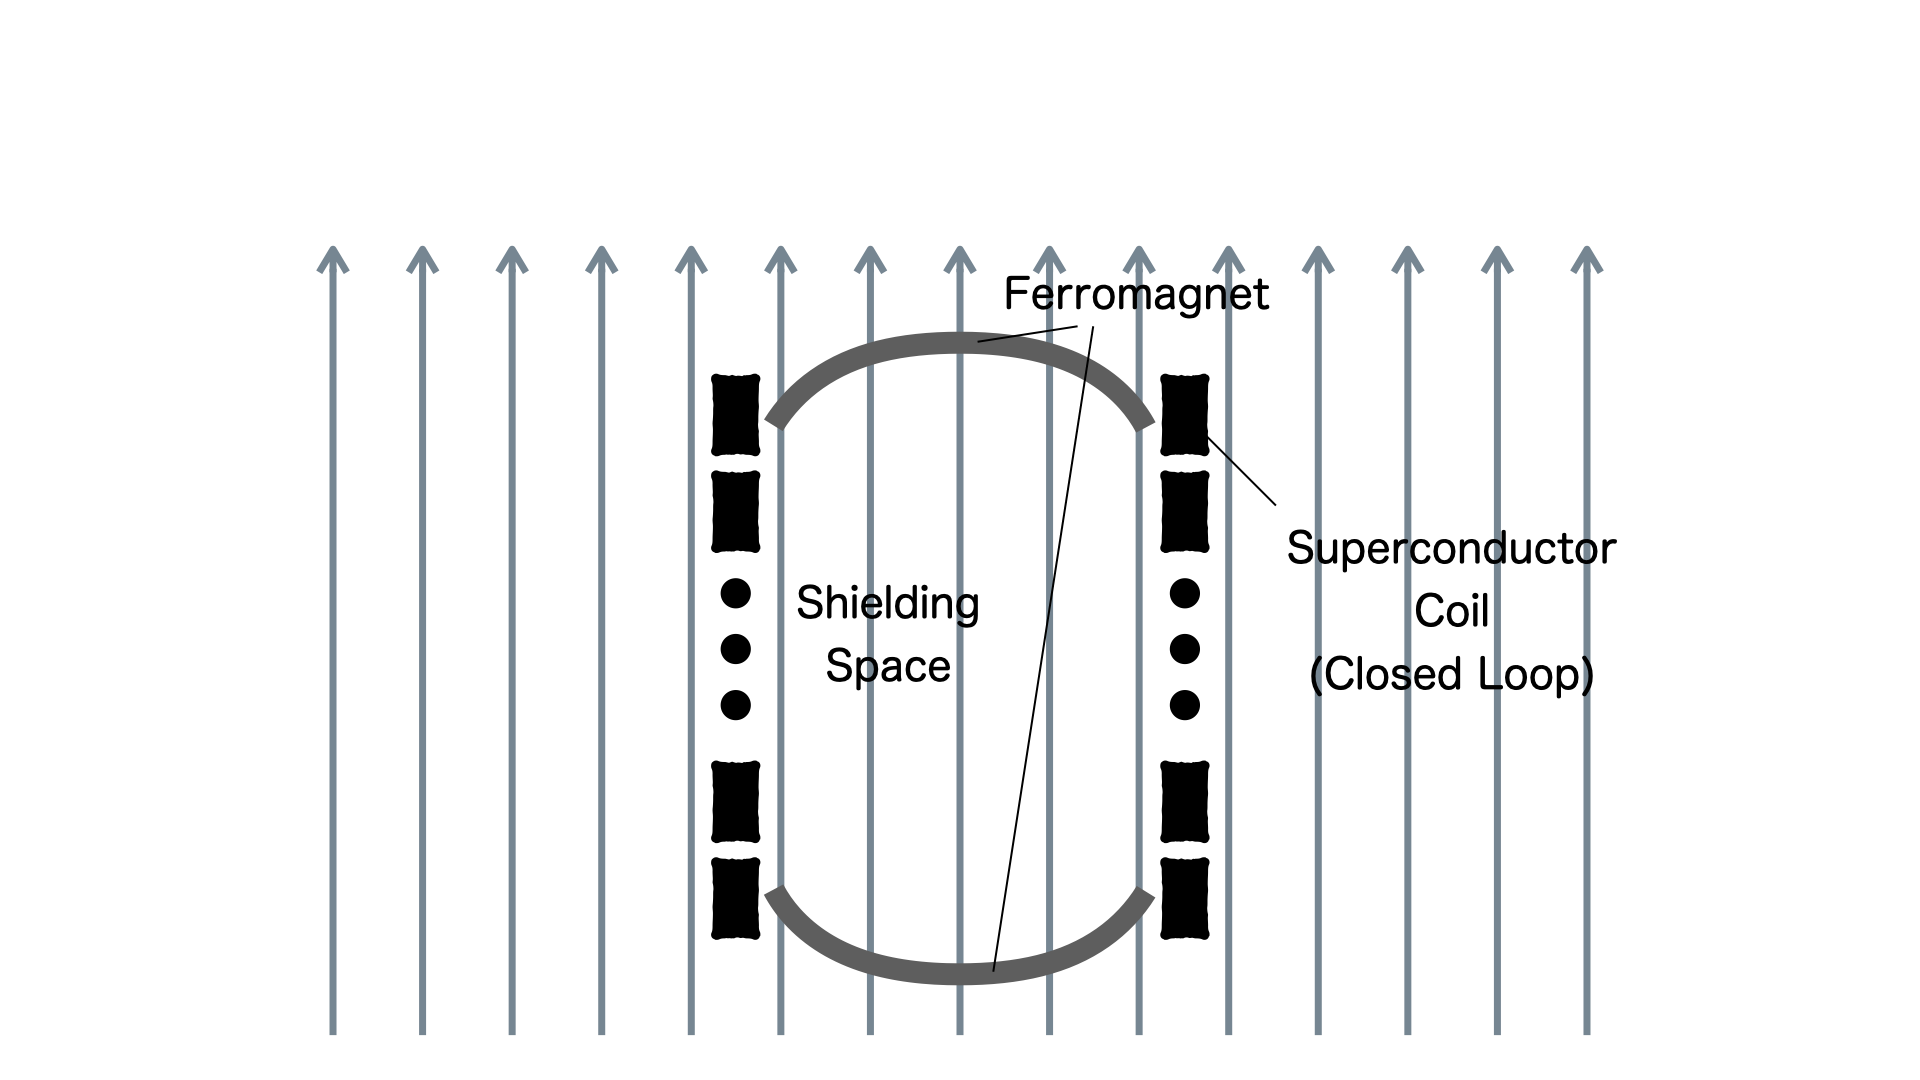
\includegraphics[width=13cm, bb=9 9 900 550]{./section2Proposal/EMIC1.png}
  \caption{Solenoid superconductor windings imposed by external field (before).}
  \label{fig:EIMC1}
\end{figure}
\begin{figure}[H]
  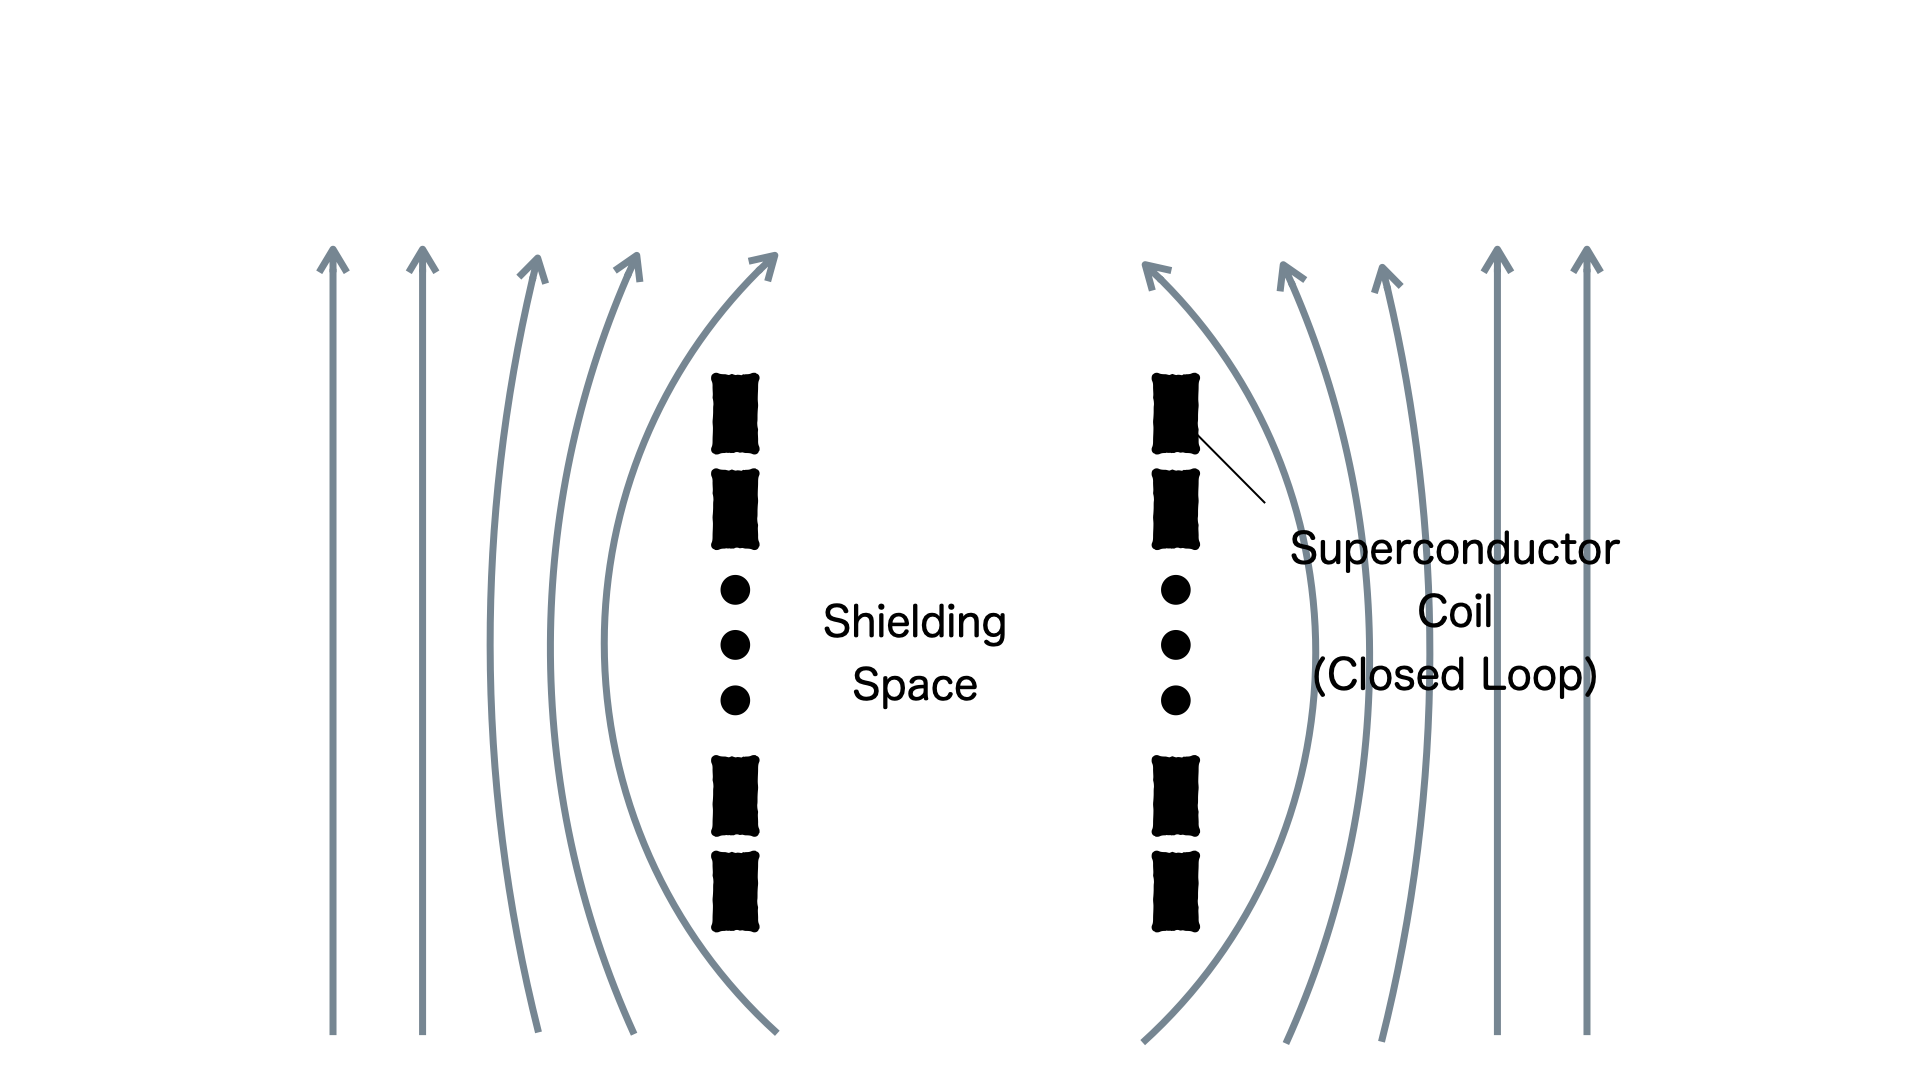
\includegraphics[width=13cm, bb=9 9 900 550]{./section2Proposal/EMIC2.png}
  \caption{Solenoid superconductor windings imposed by external field (before).}
  \label{fig:EIMC2}
\end{figure}
\begin{figure}[H]
  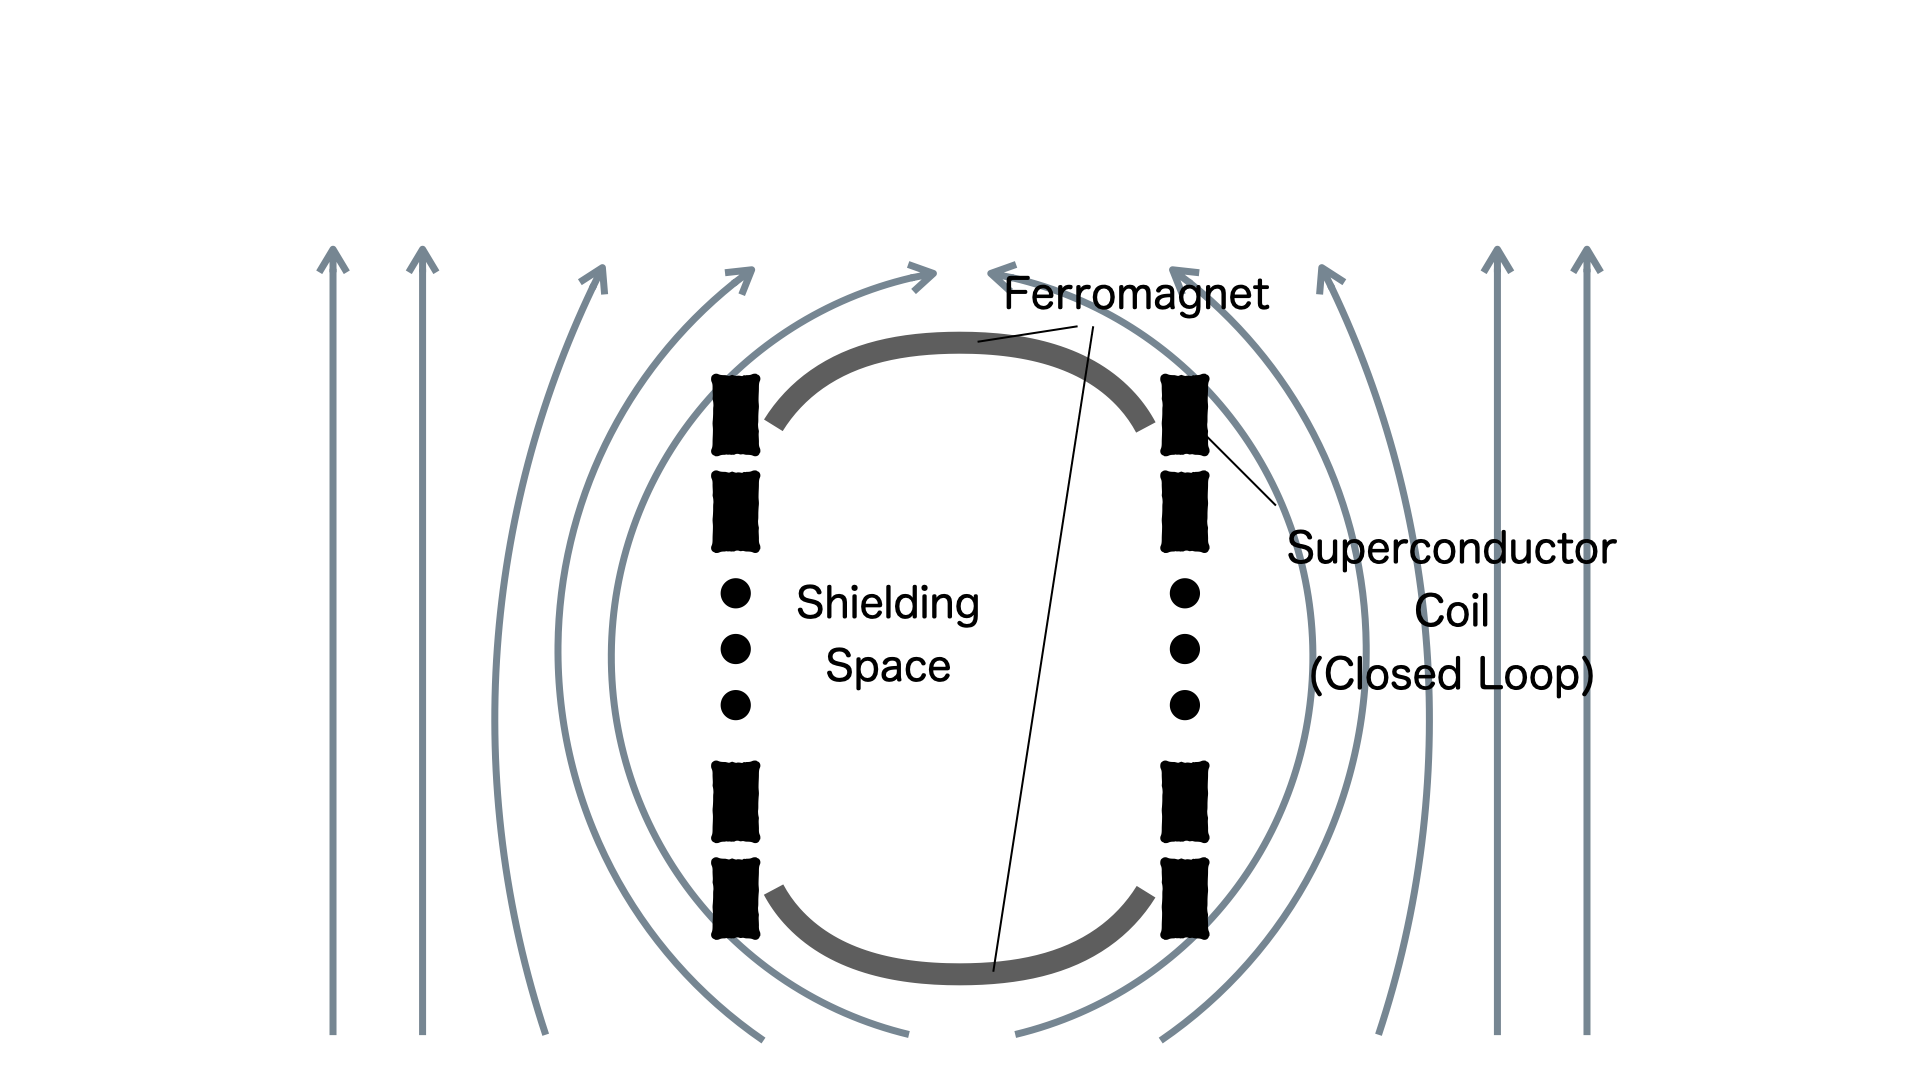
\includegraphics[width=13cm, bb=9 9 900 550]{./section2Proposal/EMIC3.png}
  \caption{Adding ferromagnet on the edge of the coil should reinforce the outer field near the edge.}
  \label{fig:EIMC3}
\end{figure}
If we impose magnetic field from the external,
since the tapes are closed and in the superconducting state,
huge permenant current would be induced,
canceling out the external field (Fig. \ref{fig:EIMC1}$\to$Fig. \ref{fig:EIMC2}).
Moreover, if ferromagnets are placed on the top and bottom edge additionally,
the outer field would be reinforced by the strong magnetization.
Since more turns the superconductor windings is made of,
more canceling field can be generated,
which gives the model full scalability to high fields.
We have named this model "Electromagnetic Induction Type" to distinguish it from the conventional magnetic cloak using Meissner effect.

With this concept, a shielding system with cloaking property capable of working under high field environment can be expected.
In the following chapter, we show the studied effectiveness of it.


\newpage
\begin{thebibliography}{20}
  \bibitem{2_1} Fritz London, "Superfluids I, Macroscopic Theory of Superconductivity" (1950)
  \bibitem{2_2} H. Kamerlingh Onnes, Leiden Comm., 122 b, 124 c (1911)
  \bibitem{2_3} D. B. Cook, M. W. Zemansky, and H. A. Boorse, Phys. Rev. 78, 820 (1950)
  \bibitem{2_4} H. Kamerlingh Onnes and W. Tuyn, Proc. Acad. Sci. Amsterdam, 25, 443 (1923)
  \bibitem{2_5} W. Meissner and R. Ochsenfeld, Naturwissenschaften, 21, 787 (1933)
  \bibitem{2_6} J. G. Bednorz and K. A. Müller, "Possible highTc superconductivity in the Ba−La−Cu−O system", Z. Physik, B 64 (1), p. 189–193 (1986)
  \bibitem{2_7} Pia Jensen Ray. Figure 2.4 in Master's thesis, "Structural investigation of La2–xSrxCuO4+y - Following staging as a function of temperature". Niels Bohr Institute, Faculty of Science, University of Copenhagen. Copenhagen, Denmark. (2015)
  \bibitem{2_8} Drozdov, A. P.; Eremets, M. I.; Troyan, I. A.; Ksenofontov, V.; Shylin, S. I., "Conventional superconductivity at 203 kelvin at high pressures in the sulfur hydride system", Nature. 525 (7567): 73–76. (2015)
  \bibitem{2_9} Snider, Elliot; Dasenbrock-Gammon, Nathan; McBride, Raymond; Debessai, Mathew; Vindana, Hiranya; Vencatasamy, Kevin; Lawler, Keith V.; Salamat, Ashkan; Dias, Ranga P., "Room-temperature superconductivity in a carbonaceous sulfur hydride", Nature. 586 (7829): 373–377 (Oct. 2020)
  \bibitem{2_10} London, F. (September 1948). "On the Problem of the Molecular Theory of Superconductivity", Physical Review. 74 (5): 562–573 (1948)
  \bibitem{2_11} J. Bardeen, L. Cooper and J. R. Schrieffer, "Theory of superconductivity", Phys. Rev. 108 1175 (1957)
  \bibitem{2_12} Shiro Sakai, Marcello Civelli, and Masatoshi Imada, "Hidden Fermionic Excitation Boosting High-Temperature Superconductivity in Cuprates", Phys. Rev. Lett. 116, 057003 (2016)
  \bibitem{2_13} Edward M. Purcell, "バークレー物理学コース 電磁気 復刻版 (Berkeley Physics Course Electricity and Magnetism)" (2013)
  \bibitem{2_20} Fedor Gömöry et al., "Experimental Realization of a Magnetic Cloak", Science 335, 1466 (2012)
\end{thebibliography}
